\chapter{Introduction}
\label{Introduction}

Audio processing, more precisely named audio signal processing, has been of interest since radio broadcasting and telephone systems capable of sound transmission started to replace the morse code\cite{spanias2006audio}. In it's simplest form, as used in the original telegraph, morse code is created by repeatedly opening an electrical circuit manually with a switch so that a visualisation device like a light bulb or an electric bell is turned on and off intermittedly. This discrete signal is transmitted over distance by extending the electrical circuit with long wires to a different physical location, so that the switch operator can transmit a message by morse encoding to the recipient who will have to use the same codebook for decoding.

\begin{figure}[h]
    \centering
	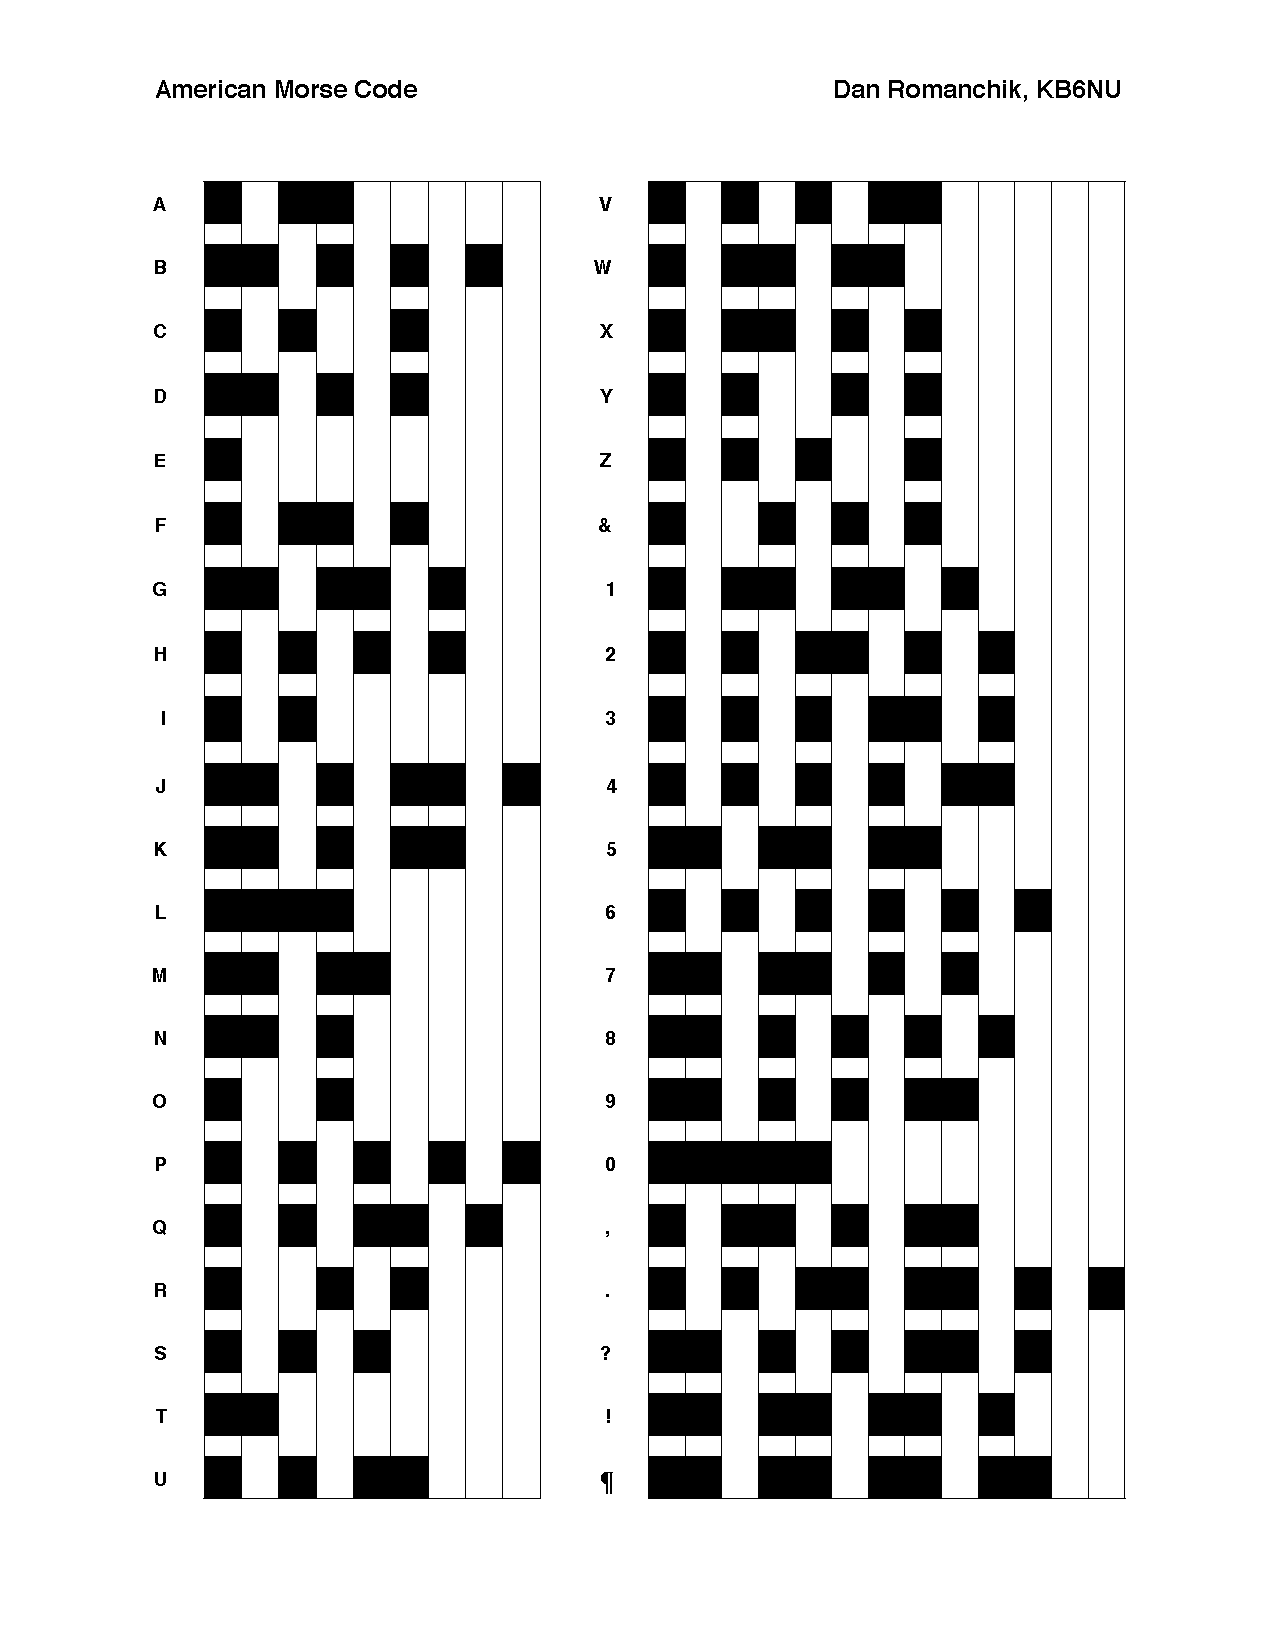
\includegraphics[width=.45\textwidth]{./images/illustrations/morse-chart}
    \caption{A codebook for the international morse code, where black means transmit}
    \label{fig:morse}
\end{figure}

The same purpose can be achieved wirelessly by repeatedly turning a radio transmitter on and off, which can be considered the simplest form of HF-modulation. However, things are more complex for the real- or near-time transmission of speech without manual en- and decoding. Since most harmonics of the human voice occur in the range of 500 Hz to 2 kHz, according to the Nyquist–Shannon sampling theorem a sampling rate of at least 4 kHz is required for transmission\footnote{To verify this empirically I have downsampled a recording of both my voice and of the song Tom's Diner to 4kHz. While both the voice and the lyrics were still understandable, the melody perished and the sounds F and S were nearly indistiguishable. This is probably the reason why many speech encoding standards like the common G.711 use a sampling rate of 8 kHz}. When radio transmission was invented in the late 19th century, it was not feasible to encode this information in a digital form (such as morse code). Instead different forms of analog modulation methods had to be developed, which was the birth of audio signal processing.

\begin{figure}[h]
    \centering
	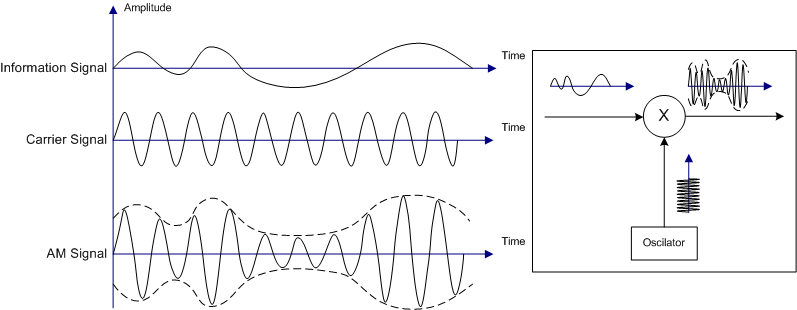
\includegraphics[width=.85\textwidth]{./images/illustrations/am}
    \caption{Amplitude modulation. Created by Ivan Akira. Source: Wikipedia; CC-BY-SA}
    \label{fig:am}
\end{figure}

From the early 20th century onwards it started to transcended it's original use while still being required for every form telecommunication. The grammophone necessisated frequency alterations for more natural sound and the development of cinemas lead to improvements in speaker technology, separation of tweeter and woofer and required the invention of crossover networks \cite{spanias2006audio}.
Today it is widely used for purposes such as entertainment (iPod), medical devices (ultrasound systems), magnetic storage of information (audio cassette, hard disks), and speed measurement (doppler effect).
 
 
Before computers enabled digital signal processing, audio was handled transformed with discrete analog circuits. An equalizer for example was constructed by using resonant circuits (consisting of an inductor and a capacitor) as a frequency filter to allow independent gain control with separate amplifiers for different bands.
There are several different areas of audio processing such as sound effects, modulation and demodulation, compression, and quality enhancements like noise reduction.

An especially interesting area of audio processing is classification.  Given an audio sample, choose the best-fit class for that sample from a finite set of classes.  A common usage is music genre classification (and other music information retrieval tasks), with the purpose of finding the genre a music sample belongs to. In this thesis my specific focus is on urban sound classification: given an audio sample, choose which class, for example, police sirens, car horns, motorcycle engines or other sounds that occur in natural urban environments the sample belongs to. This problem has several applications such as increasing the safety of self driving cars by detecting the existence and direction of car sirens before the car itself becomes visible or measuring the health impact of different forms of noise on the population.

The first project idea was to assist MIT AgeLab's human factors research in the traffic safety impact of self driving cars. This lab has a long history of detecting different forms of driver frustration with monitoring equipment in cars. They have also published research on the automatic detection of these factors through machine learning on video and audio \cite{Abdic:2016:DFD:3060621.3060809} instead of manual annotation.


\begin{figure}[h]
    \centering
	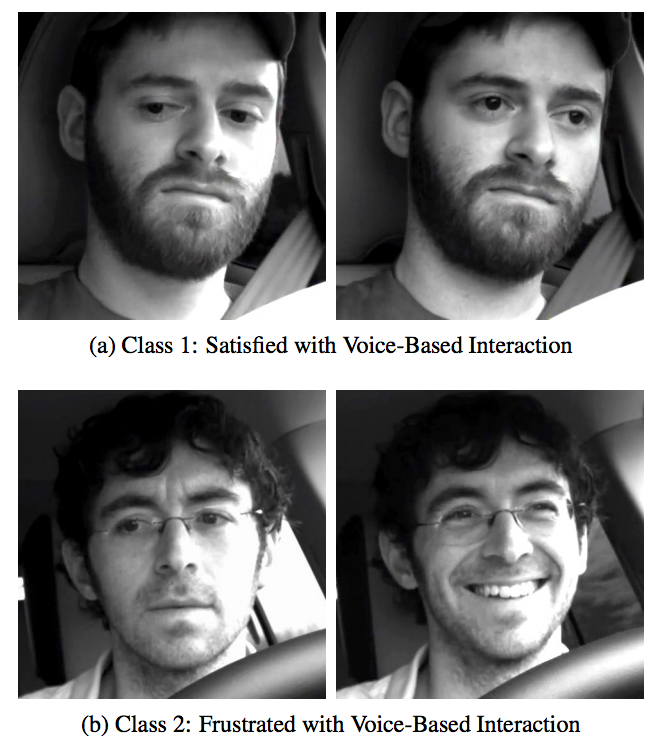
\includegraphics[width=.65\textwidth]{./images/illustrations/driver-frustration}
    \caption{Different examples of concentration and frustration while interacting with an in-car voice control system as shown in \cite{Abdic:2016:DFD:3060621.3060809}.}
    \label{fig:am}
\end{figure}


Machine learning is especially interesting as an addition in the field of audio processing. Previously this has mainly seen popularity in the audio processing task of speech recognition. While there have been many advances in this area, there has been surprisingly little work in other audio processing tasks, for example, in the detection of urban sounds and background audio classification in general. Until recently, these tasks have been approached using sophisticated, hand-crafted features and algorithms that mostly have existed since the sixties or earlier and were optimised to take advantage of analog hardware. As hardware advanced, more modern algorithms and techniques were able to be used such as gradient boosting and neural networks. These approaches represent the current state-of-the-art as it applies to audio classification.


%% WHAT DID NOT MAKE IT INTO THE THESIS
During this project software was created to automatically detect different sounds, most important the Tesla Autopilot's 'immediate takeover alarm`. I also attempted to use the developed detection of car horns to create a geogrpahic dataset of areas with high driver frustration and see if that could be correlated with accident statistics. However the available dataset of recorded traffic audio with position information turned out to be insufficient for this task.

The main purpose of this thesis then was to apply state-of-the-art neural network architectures and feature extraction to the task of urban sound classification using the UrbanSound8K dataset created by J. Salamon, C. Jacoby and J. P. Bello for the Sounds of New York City project \cite{Salamon:UrbanSound:ACMMM:14}. In this regard, I discuss several popular neural network architectures, such as CNNs, LSTMs, and attention mechanisms, and their performance in regards to audio classification. Specifically this thesis explores the use of LSTMs in urban sound classification, both with and without attention mechanisms. Furthermore, the results are compared to the use of gradient boosting and other existing algorithms against the same dataset.

%% Compared to results of the original papers



\chapter{Background and Related Work}
\label{Background and Related Work}

Although there have been some recent breakthroughs in the field by Google's Deep Mind project (\cite{DBLP:journals/corr/OordDZSVGKSK16}) raw audio is rarely used  with machine learning algorithms directly. This is because one minute of mono channel audio, sampled with the very common AD conversion rate of 44.1 kHz, produces the amount of 2.646.000 data points alone. The data points are usually 16 bit integers indicating the amplitude of the audio wave at the present moment.


\begin{figure}[h]
    \centering
	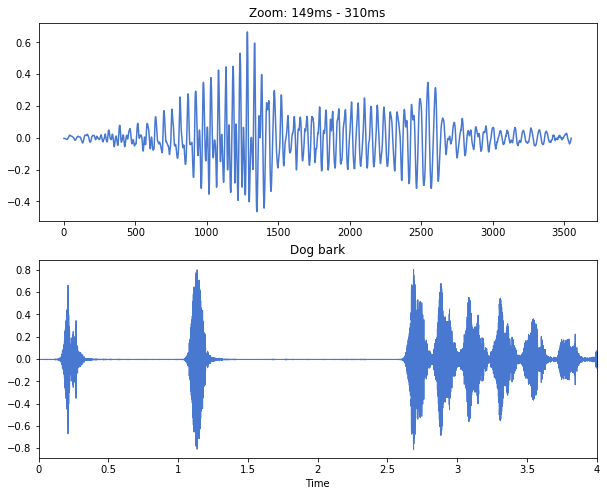
\includegraphics[width=.85\textwidth]{./images/illustrations/audio-signal}
    \caption{Common wave-plot representation of a 4s dog bark audio file and a zoom into seven 23ms frames consisting of 3549 data points}
    \label{fig:audio}
\end{figure}


This is in stark contrast to the amount of data in other machine learning tasks, such as the common 28x28 greyscale image in the MNIST image recognition dataset, where each image is represented by only $28*28*8 = 6.272$ bits \cite{lecun1998mnist}.

Therefor we rely on a mechanism called feature extraction. This means the creation of a signal processing algorithms, that transforms the raw audio signal into meaningful information, by removing redundancies and irrelevancies while presenting the relevant information in as little dimensions as possible. A challenge is that what might be relevant differs strongly depending on the context. As an example, the well-known MP3 compression specifially removes content that can not be heard by the human ear \cite{brandenburg1999mp3}. While that is adequate for digital compression of an audio file without affecting the  listener's impressin, this might very well decrease the detection and classification rate of other algorithms.  


\section{Machine Learning for Audio through Feature Extraction}


[wtd list and describe various audio processing task such as sound classification and speech recognition]

[wtd describe historical approaches to audio classification and audio processing tasks]


For the purpose of this thesis, I have evaluated the ESSENTIA audio analysis library \cite{bogdanov:Essentia:ACMMULTIMEDIA13} via its Python bindings and librosa \cite{BMcFee:librosa}, which is a native python implementation. 
These have been selected as they seem to be the only actively-maintained open-source packages for audio signal processing with sufficient background literature and documentation. 

Later, my supervisor suggested to compare the results to OpenSMILE, which is promoted as the "Munich Open-source Multimedia Feature Extractor" \cite{Eyben:2013:RDO:2502081.2502224}.
OpenSMILE is extremely easy to use through its command line tool "SMILEextract". A simple demo script that extracts some basic features can be created by invoking "SMILExtract -cfgFileTemplate -configDflt cWaveSource,cFramer,cEnergy"\footnote{This example taken from the OpenSMILE manual extracts log energy features broken down into separate frequency bands. There are configuration examples for Chroma, MFCC, and PLP features delivered with the library.}.
The resulting csv can be read with python csv script and very often directly be used for machine learning applications. While this library has proven to be extremely powerful, the  configuration procedure and the multi-step pipeline led me to prefer librosa, so that everything from loading the audio, to feature selection and extraction as the machine learning steps could be implemented in python.  %TODO: Different results with librosa and OpenSMILE.

\subsection{Spectrograms}

Probably the best-known feature extractor is the Fourier Transformation. In 1822, while studying heat transfer, Joseph Fourier proved that certain functions could be written as a sum of a finite number of harmonics \cite{fourier1878}. This led the way onto the development of the Fourier transform, the decomposition of a signal into the different sine frequenices it is made up of. As input, the Fourier transform requires a periodic and infinite signal. In real-world scenarios, where recorded instead of generated input is used, the signal is cut into short slices and the transformation is done for each slice individually with the assumption that it would be repeating indefinitely as a simple workaround \cite{Smith97}.

The advance of digital signal processing has made it possible to utilize the Fourier transform to create a visual representation of the different frequencies in a signal such as sound. The most common format of display is a a two-dimensional diagram, where the abscissa represents the time dimension and the ordinate the separate frequency ranges. The intensity can either be displayed through the brightness or intensity of different colors. 

\begin{figure}[h]
    \centering
	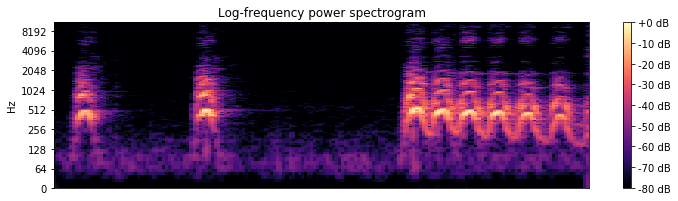
\includegraphics[width=.9\textwidth]{./images/illustrations/spectrogram}
    \caption{The spectral distribution of the dog bark audio}
    \label{fig:spef}
\end{figure}

To increase verboseness and to prevent noise, individual slices can be created overlapping through the use of window functions. Subsequently the intensity of each spectrum can be calculated by applying the fourier transform onto the thereby generated individual chunks.


\subsection{MFCC}

In Indo-European languages a change of the pitch usually does not alter a spoken word’s meaning \cite{auditoryneuroscience}. Instead, information is encoded by filtering the sound while passing the vocal tract, including the pharynx and the tongue causing changes in the envelope of the short time power spectrum. This makes the fourier transformation itself not helpful with speech recognition. Other information, like the speaker's gender and nervousness could possible be extracted nevertheless.

That is why a method has become extremely popular that provides a separation between voice pitch and the formants. Developed by \cite{noll67}, the Mel-frequency cepstral coefficients (MFCCs) have become the most commonly used feature in speech recognition tasks \cite{ganchev2005comparative}, a transformation that is inspired by the inner workings of the cochlea, including the sensory organ of hearing inside the human ear, the Organ of Cortil. 

\begin{figure}[h]
    \centering
	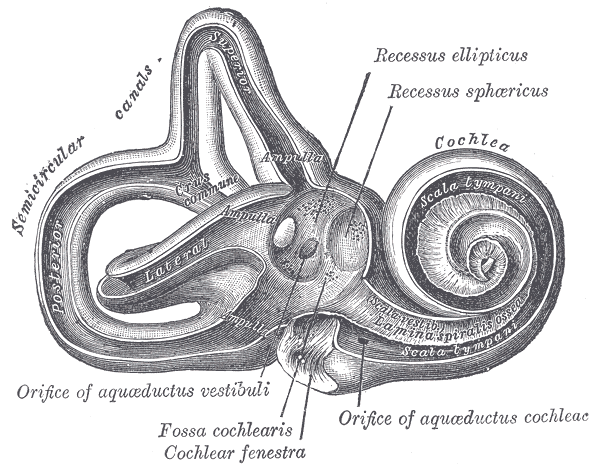
\includegraphics[width=.7\textwidth]{./images/illustrations/Gray921}
    \caption{Location and principle of the cochlea inside the inner ear. - Henry Gray, 1918, copyright expired}
    \label{fig:gray}
\end{figure}


The first step in its calculation is the slicing into short frames through a window function, mimicking inertia in the organ. Different sound frequencies create resonance in different areas of the cochlea’s narrowing spiral tube, where the wobbling of sensory hair called the stereocilia create nervous impulses.

To identify the different frequencies, the next step is the calculation of a power spectrum through Fourier transformation. This result is a power spectrum on a linear frequency scale, which does not correlate well with the perception of different frequencies in humans \cite{mel}. 

  \begin{figure}[h]
    \centering
	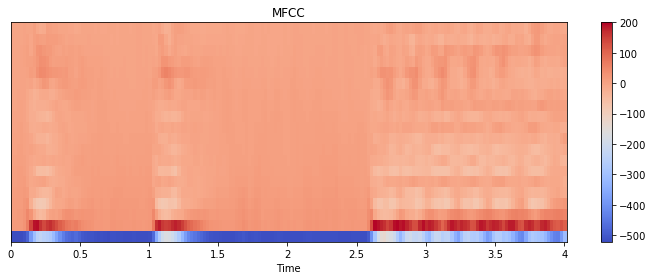
\includegraphics[width=.6\textwidth]{./images/illustrations/mfcc}
    \caption{Graphic representation of MFCCs of the dog bark audio file}
    \label{fig:mfcc}
\end{figure}
 
 
 While low frequencies below 20 Hz can hardly be detected, the effect becomes especially predominant with frequencies over 1 kHz. The transformation from the Hertz- onto the so-called Mel-scale is used as the next step to map the spectrum onto the percieved frequencies. 
 
 The linear scale is mapped into discrete bins through a triangular activation functions within the human hearing range as well in this step. Like most human senses in accordance to Fechner’s law \cite{fechner1860} the relationship between stimulus and perception is logarithmic, wich means a quadrupling of the acoustic pressure causes the perceived intensity (loudness) of sound to double. A similar effect can be achieved by taking the logarithms of the power spectrum.
 

 To decorrelate the energies of the overlapping filterbanks, in order to separate pitch, modulation (added by the vocal in human speech) and noise, usually the discrete cosine transformation is performed on the log mel powers. % The resulting coefficient 2-13 form the MFCCs.
 
 The resulting amplitudes form the Mel-frequency cepstral coefficients.

\subsection{Chroma}

The chroma feature is mainly used in music recognition. It is based on the twelve pitch classes commonly used in music theory \cite{Mller:2015:FMP:2815664}. Sounds that differ by one or more octave, i.e. ratio of frequencies occur at a ratio of $2^n : 1$ with n being an integer.


\begin{figure}[H]
    \centering
	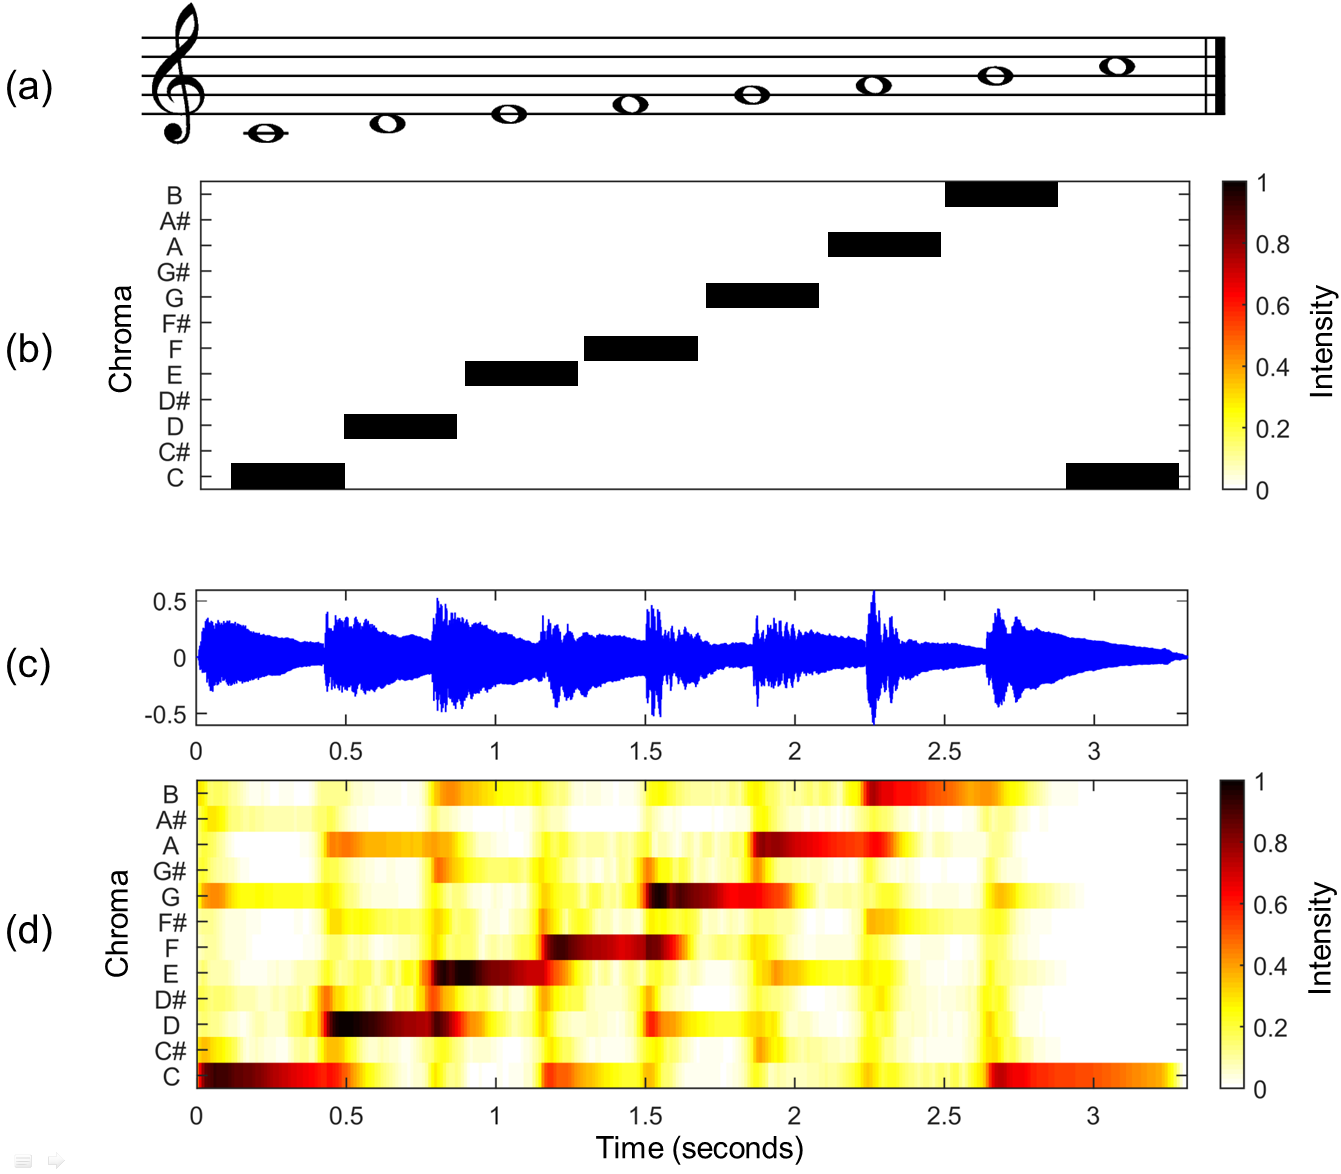
\includegraphics[width=.5\textwidth]{./images/illustrations/chroma}
    \caption{Illustration of the Chroma feature of a C maj scale played on a piano. Created by Meinard Müller. Source: Wikipedia; CC-BY-SA}
    \label{fig:chroma}
\end{figure}



\section{Traditional machine learning approaches}


Machine learning has once more become popular in the last few years as the recent advancements supplied sufficient computational power for training deep neural networks with huge amounts of data.
It can mathematically be described as a system that receives existing data and generates a function that can be used to predict properties of future data.
The quality is measured as the generalization performance, i.e. the accuracy on data used not for training.


There are multiple different machine learning algorithms useable with audio information recognition.


\subsection{Linear and Logistic Regression}


 
The simplest model of a relationship between an explanatory and one dependent variable is the linear regression with a dataset ${\displaystyle \{y_{i},\,x_{i}\}_{i=1}^{n}}$ of n statistical units, with Y being the dependent and x being the explanatory variable.
The model is then calculated based on a linear predictor function where the parameters for slope and intercept are estimated by using the available data.
 
The model is not restricted to a single explanatory variable, where the data set can be described as  ${\displaystyle \{y_{i},\,x_{i1},\ldots ,x_{ip}\}_{i=1}^{n}}$. When multiple explanatory variables are used, the model is referred to as multiple linear regression, where the model will take the form of ${ y_{i} +\varepsilon _{i} =\beta _{0}1+\beta _{1}x_{i1}+\cdots +\beta _{p}x_{ip}}$ with $\varepsilon$ being the error parameter sought to be minimised.

There are multiple ways of estimating the parameters available, with the conditional mean being the most frequently used function, while the median and other statistical qualtiy functions are less common \cite{Yan:2009:LRA:1717831}.  $\varepsilon$ is commonly calculated over the sum of the squared euclidian distances from each Y from the predicted value.


Although simple, multiple linear regression is used extensively for a variety of tasks in practice, for example in Germany to estimate the credit risk of consumers (Schufa) with parameters being the length of the credit histroy, the frequency of address change and the number of different credit cards and bank accounts on one customer. % TODO: Cite


Another generalisation of this concept, where multiple dependent variables are predicted, is the extension of the process called multivariante linear regression. All dependant variables need to be correlated however \cite{Yan:2009:LRA:1717831}.


For discrete choice or other distributions where the dependent variable is a discrete or binary category, the modified version called logistic regression was developed in \cite{cox58reg}. Instead of a linear model, the  function ${\displaystyle F(x)={\frac {1}{1+e^{-(\beta _{0}+\beta _{1}x)}}}}$ will always return a value between 0 and 1, which can be interpreted as the likelihood of a dataset falling into the binary category labeled as 1. It also allows to estimate the relationship of an explanatory variable and the likelihood of an outcome (e.g. speeding will increase the likelihood of an accident by xx\%)

Parameter estimation is hereby more complicated than in linear regression and an iterative method needs to be used, such as the Newton–Raphson method.

%rule of 10 ?

The primary downfall of linear/logistic regression is the inability to model non-linear relationships. These are very common in nature, famous examples are the half-life of radioactive decay or the exponential growth of most biomass.


\subsection{SVMs}


Support Vector Machine are among the most popular supervised machine learning methods and have shown great success in the classification of high-dimensional data. In its simplest form a model is created out of training data, with each instance belonging to one of two categories and the categories are linearly separable.


\begin{figure}[h]
    \centering
	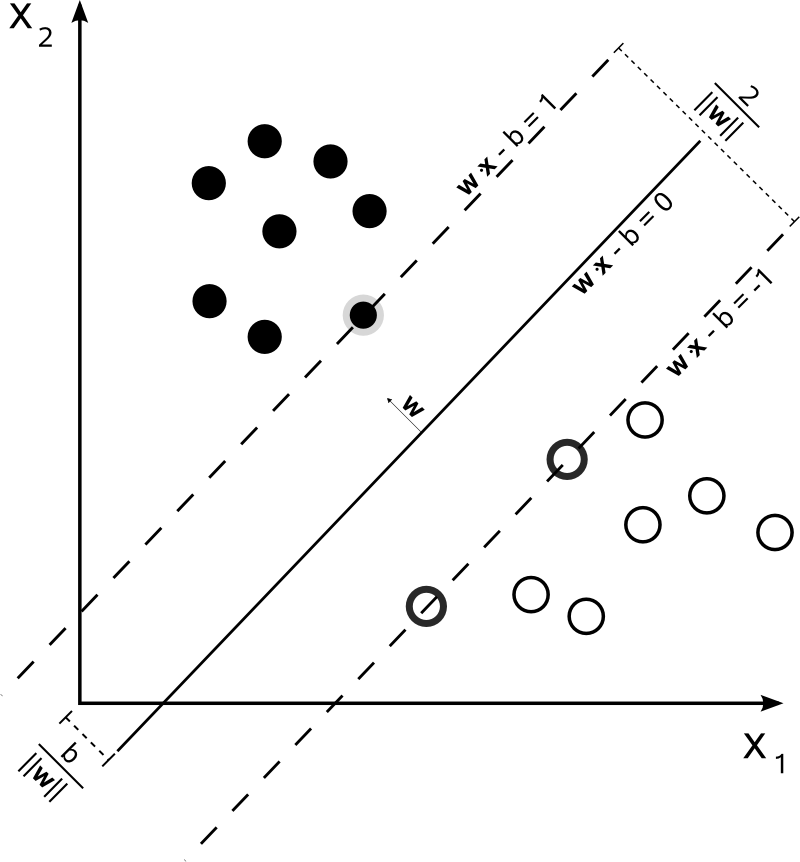
\includegraphics[width=.5\textwidth]{./images/illustrations/svm}
    \caption{Example of linear separation of two classes on maximum-margin hyperplane. Source: Wikimedia Commons; Public Domain}
    \label{fig:svm}
\end{figure}

The biggest improvement in SVMs over more traditional machine learning methods is that it will find on optimal solution without being affected by local minima.

Support vectors are the subset of all data points lieing closest to the decision surface (as seen in figure \ref{fig:svm}). These specify the decision function entirely by themselves. The SVM optimizes the margin around the separating hyperplane (a line in 2 dimensional space) to be maximum.

By using a kernel function, they can be extended onto categories that are not linearly separable. The kernel will transform the original input space that may be non-linear and of higher dimension into a simpler space that can be linearly separated with a hyperplane. Known kernels are available for polynomic, hyperbolic tangent and other relationships. However choosing the right kernel may not always by easy and trial and error with cross validation is sometimes necessary.

They can be used for classification as well as for regression.


%TODO: citations needed



\subsection{Random Forests}


Random forest classification was introduced with \cite{Breiman2001} and have shown success in predicting medical events, such as developing certain diseases as there are multiple advantages over other classification methods like SVM.

The random forest classifier is a predictive model consisting of multiple decision trees. The risk of overfitting the model to the available data, but not generalising well to new data is significantly reduced by learning multiple models over different subsamples of the training set and casting a majority vote at prediction time. \cite{statisticallearning}.

The first step in growing a forest is the creation of $n$ random subsamples of the training data, which are allowed to overlap. Each subsample is used to create an independent decision tree, where a small number of features is randomly selected that may be considered as the predictor for each split until the tree is fully developed.

Like other machine learning methods, random forests can be used for regression, if instead of decision trees regression trees are computed and the majority vote is replaced with averaging the result of the trees. However, the performance of using the random forest algorithm for regression has shown to fall behind other methods and it is therefor seldomly used.

A big advantage of this algorithm is that empirical data suggests that the out-of-bag error estimate is almost identical to that obtained by cross-validation, which means it is unlikely that overfitting might have skewed the results. Other advantages are that the evaluation can be parallelised very efficiently through map-reduce, as each tree can be evaluated independently. This makes it very efficient on big amounts of data. Also the training effort only scales linearly with the number of trees, which leads to fast iterations.

These characteristics make random forests useful for audio classification, where the available datasets are usually limited and other algorithms might overfit to certain characteristics of the recording equipment instead of the recorded data.

%TODO: higher accuracy on smaller dimensional data or datasets

%TODO: pitfalls of random forests

%TODO: estimators to features 



\subsection{Gradient Boosting}

Gradient boosting is an supervised ensemble learning method that combines many "weak" learners, to form one single strong learner.  It has been proven to be a very successful machine learning method and has been applied with great success to many different challenges of the machine learning competition "Kaggle". Like most methods, it can be applied to both regression and classification problems.

The concept of Adaptive Boosting was introduced with \cite{Freund97adecision-theoretic} Freund and Schapire and has become the classic example of learning with boosting. It sequentially trains a serious of models that are able to accept a weighted collection of training points, i.e. we would add a vector of weights to our training data that indicates the importance of accurately predicting each specific data point. In each sequence the importance of incorrectly predicted data points is increased and the weight of the ones predicted correctly decreased and therefor incrementally minimizing the exponential loss.

An unwanted side effect of this boosting technique is that very often the weight of statistical outliers is increased continously and noise is amplified heavily. Adaboost therefor depends on high-quality. % data and experiments during this thesis have not been proven to give useful results TODO: Detail this

The library xgboost \cite{DBLP:journals/corr/ChenG16} has become the de facto standard for gradient boosting after winning Kaggle's Higgs Machine Learning Challenge in 2014 \cite{xgboost-wins}. While there are nowadays bindings for nearly any language available, only the integration into Python's scikit-learn has been evaluated for this thesis.



\section{Neural Networks}

Contrary to the previously discussed approaches to machine learning, neural networks have existed for much longer. Surprisingly, the idea of creating a mathematical model of an artifcial neuron has first been published in 1943 \cite{McCulloch1943} with the intent of studying whether a mammalian brain could truly evaluate computable mathematical functions.

In this paper each neuron is a function with one binary output $y \epsilon \{0;1\}$ and one or multiple binary inputs $x_n \epsilon \{0;1\}$ with a specific weight $w_n \epsilon \mathbb{R}$ and a threshold value $T \epsilon \mathbb{R}$. A weighted sum of inputs is calculated with the simple arithmetic operation $\text{sum} = x_1w_1 + x_2w_2 + x_3w_3 + ...$ . The output value is dependent on the neuron's threshold

{\centering
	$y(x_1, ..., x_n) = \begin{cases}
    0,& \text{if } \text{sum} < T\\
    1,& \text{if } \text{sum} \geq T\\
	\end{cases}$
	\par
}

This allows for the modeling of boolean AND-, OR-, and NOT-relationships, making a network of McCulloug-Pitts neurons forming a full equivalent to the boolean algebra. Consequently the authors already assumed, that nearly every arithmetic function could be calculated with generalisation of this concept form binary in- and outputs to real numbers. This is done in modern neural networks, by replacing the threshold with an activation function (see \ref{activation}).


\begin{figure}[h]
    \centering
	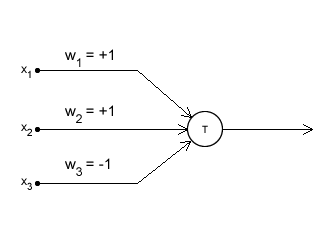
\includegraphics[width=.6\textwidth]{./images/illustrations/mcculloch-pitts}
    \caption{Graphical representation of the McCulloch-Pitts model. Source: aishack.in}
    \label{fig:mcculloch-pitts}
\end{figure}


 Neural networks have had a fickle history as well, with an ebb-and-flow of popularity, last peaking in the 90s \cite{Bengio91z}.  Due to advances in computational power, parallel processing paradigms, and neural network architectures in the past several years, neural networks are seeing great successes across many machine learning tasks. For example, in \cite{Silver:2016aa} neural networks were for the first time in history able to outperform a human champion in the game of Go, playing at a level previously thought not possible and still leaving many experienced players baffled.  


 
% explain what neural networks are, put graphs, explain advantages such as ability to deal with curse of dimonsionality and ability to deal with non-linear relationships, explain pitfalls


 [wtd explain stochastic gradient descent and optimizers ADAM, Adadelta, momentum, etc.]


%The newest branch in machine learning attempting high level abstactions is so called deep learning. 

Tensorflow is a library published by Google in 2014 in an effort to open-source their internal deep-learning functionalities into a universal library. While in the beginning it lacked distributed computing functionality and the support for GPGPU was poor, 


After a longer experience with Tensorflow, the browser based Convnet.js was evaluated to see if it could be used as a viable alternative for the tasks in this thesis.
While it being a java script implementation, due to the characteristics of any scripted language its performance naturally is unable to match the GPGPU accelerated TensorFlow implementation, where Python only serves as high-level bindings in order to simplify the API interface and its implementation in real world use cases.tens

It's strength primarily 


Hacker's guide to Neural Networks: http://karpathy.github.io/neuralnets/

GOOGLE CLOUD BIG DATA AND MACHINE LEARNING BLOG - Learn TensorFlow and deep learning, without a Ph.D.: https://cloud.google.com/blog/big-data/2017/01/learn-tensorflow-and-deep-learning-without-a-phd


\subsection{Activation Functions}
\label{activation}

After each neuron has calculated the sum of its weighted inputs, it passes it to a (usually non-linear) "activation" function.  There are advantages and disadvantages to different activation functions.


\subsubsection{Linear}

A linear activation function takes the weighted summed inputs to the neuron and multiplies it by a constant, giving the neuron the ability to scale the inputs.

{\centering
  $f(x)=cx$\par
}


\subsubsection{Sigmoid}
[wtd describe sigmoidal activation, include math]

{\centering
	$\displaystyle f(x)={\frac {L}{1+e^{-k(x-x_{0})}}}$\par
}

\subsubsection{TanH}

Similar to the sigmoid function, [wtd explain tanh]

\subsubsection{Rectified Linear Unit}
[wtd describe relu activation, include math]

{\centering
	$f(x)=max(0, x)$\par
}

\subsubsection{Scaled Exponential Linear Unit}
[wtd describe selu activation, include math, include special initialization required]


{\centering
	$\text{selu}(x) = \lambda\ \begin{cases}
    x,& \text{if } x > 0\\
    \alpha e^{x} - \alpha,& \text{if } x\leq 0\\
	\end{cases}$
	\par
}


The paper (\cite{DBLP:journals/corr/KlambauerUMH17})


\subsubsection{Softmax}
The softmax activation function transforms a set of probabilities

{\centering
	$\displaystyle \sigma (\mathbf {z} )_{j}={\frac {e^{z_{j}}}{\sum _{k=1}^{K}e^{z_{k}}}}$
	\par
}

\subsection{Convolutional Neural Networks}

One of the more recent improvements in the reserach of Neural Networks has been the invetion of convolutional layers, where the same form of connections between each cell of two neighouring layers is established, like a filter in a traditional programming. 

The connectivity pattern of sharing the same connectivity weights between each neurons in neighbouring layers is inspired by the visual cortex in the mammalian brain.
Mathematically, the operation can be approximated by a convolution operation, which gave the network architecture its name. 

Efforts to train the network with know filters, like the sobel image filter have been largely successful by adding before and after images.  

A special network architecture, that has proven to generate best results in image recognition is the Convolutional Neural Network \cite{Lecun98gradient-basedlearning}.
Its difference is the existence of a convolutional layer as the core building block.
Instead of having weighted connections between all the neurons in neighbouring layers the network uses a self-taught filterkernel as parameter.


Even in CNNs eventually the high level reasoning is done in a fully connected layer at the end.

AlexNet, a famous example with 500,000 neurons in five convolutional layers \cite{AlexNet} was a major breakthrough in the field of computer vision, submitted to the "Large Scale Visual Recognition Challenge 2012", which is commonly referred to as the annual olympics of computer vision.
In this competition, AlexNet achieved a top-5 test error rate of 15.4\% on the 1.2 million images in 1,000 categories, while the second best entry only achieved an error of more than 26\% \cite{ILSVRC15}. 
The network consists of five convolutional layers, includes dropout layers and employes three fully connected layers in front of the output layer. Instead of the conventional tanh activation function, ReLU makes training more efficient.
Another innovation was the parallelization happening in the training. The authors split the networks layers into separate chunks that were trained on two independent graphic cards. The training still lasted six days, even though they were using two GTX 580 GPUs, that were the most powerful solution on the market at that time.



Convolutional neural networks refers to any neural network with a convolutional layer.  These networks have achieved state-of-the-art results on many computer vision-related tasks, primarily because of their ability to "downsample" inputs while minimizing information loss.  It is because of this "downsampling" that these network are feasible to train, as opposed to a fully-connected network which has significantly more weights to train.  A convolutional layer is one that attempts to discover spatial relationships, aka filters, across neuronal inputs. [wtd describe + show graphs of convolutional layers].  This layer contains a set of filters, or weight matrices, that are convolved across the neuronal inputs, resulting in an output matrix called a feature map.  The weights of the filters are learned during training.  Typically these networks involve other spatial layers, such as max pooling layers, which directly downsample the neuronal inputs.

\subsection{Recurrent Neural Networks}

[wtd describe recurrent neural networks, cite original paper]

[wtd include math and graphs of basic RNN structure]

[wtd explain exactly the problem that RNNs solve (sequence and removing the need to include historical data in the inputs similar to how CNNs solve the problem of needing so many weights for the spatial input)]

While CNNS solve the problem of dimensionality in terms of spatial relationships, RNNs do so in terms of sequential, or temporal relationships.  Typically, to represent a temporal or sequential relationship, inputs are stacked in a windowed-fashion.  However, this greatly increases the number of weights required at the input layer.  Therefore, RNNs reduce the amount weights by allowing sequences to be passed in without requiring weights be connected to these input features.


% http://colah.github.io/posts/2015-08-Understanding-LSTMs/

While most animals have a at least one form of memory and what happened in the past is always taken into consideration, after completion of the training phase in NNs the past traditionally has no impact onto the result. 
In contrast, Recurrent Neural Network (RNNs) extend the idea by not only allowing feed-forward propagation but adding connections between units that form a directed cycle (loops), therefor allowing information to persist. 
Adding this kind of internal memory has proven to be especially useful for tasks like speech recognition \cite{sak2014long}, where due to the grammatical nature of human languages the meaning of heterograph such as to, too and two can almost always be determined by context.

While there are many different RNN architectures I have found the so called Long-Short Term Memory (LSTM) to be the most useful for the detection of driver frustration. % why?
These are especially well suited to remembering information for a long period of time, where other RNNs like the traditional single tanh layer as a repeating module very often struggle \cite{Hochreiter:1997:LSM:1246443.1246450}.




deep feed forward

multi-dimensional long short-term memory 




\subsubsection{LSTMs}

\begin{figure}[h]
    \centering
	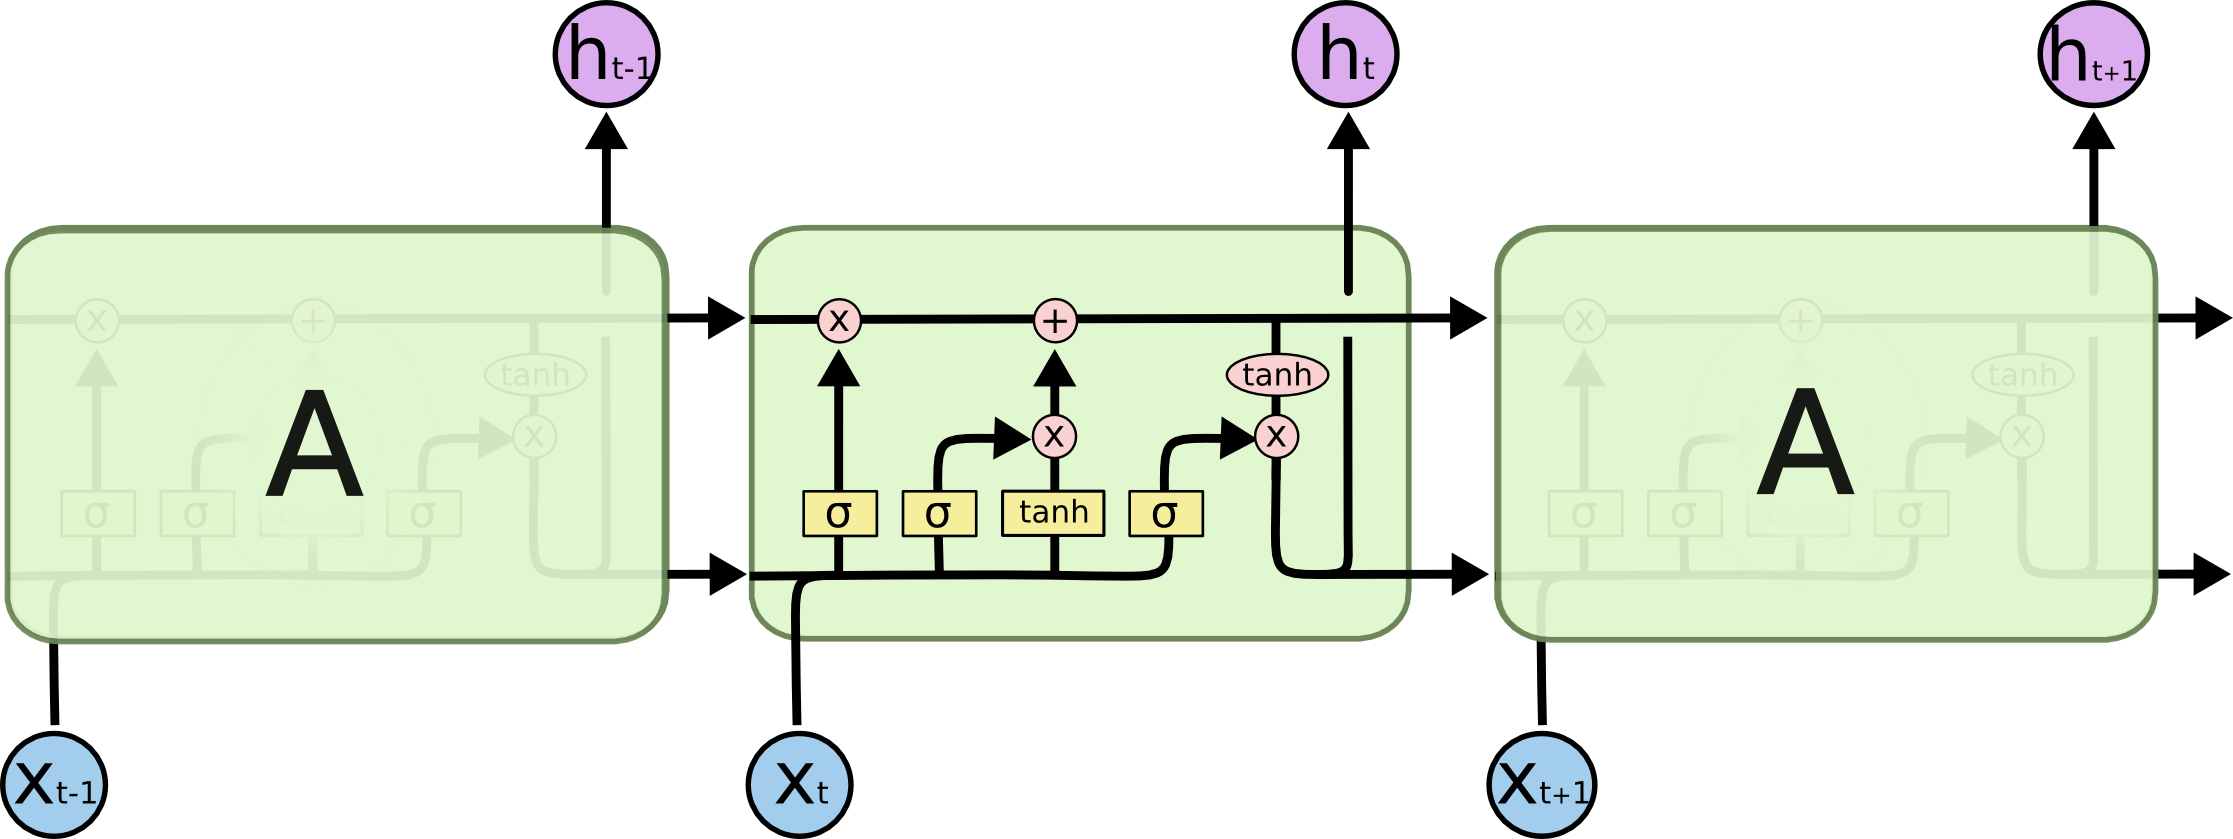
\includegraphics[width=.8\textwidth]{./images/illustrations/LSTM3}
    \caption{The repeating module in an LSTM contains four interacting layers.}
    \label{fig:mesh1}
\end{figure}\footnote{Source: http://colah.github.io/posts/2015-08-Understanding-LSTMs/. Reproduced with permission}





One of the pitfalls of recurrent neural networks is their inability to model [wtd describe lstms]

[wtd describe lstms and include graphs]

[wtd describe what problems lstms solve aka able to capture longer sequences, and downfalls]

\subsubsection{GRUs}

\begin{figure}[h]
    \centering
	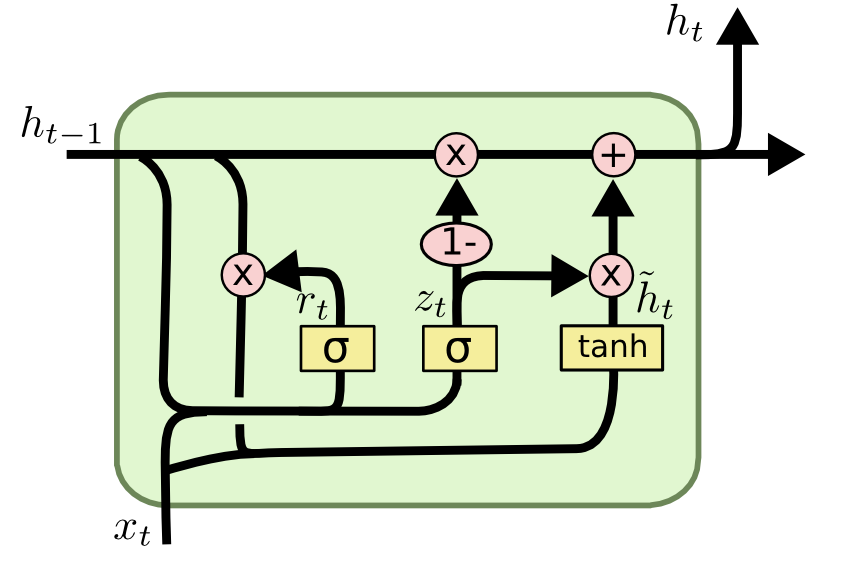
\includegraphics[width=.8\textwidth]{./images/illustrations/GRU}
    \caption{A GRU, as defined by Cho, et al. (2014).}
    \label{fig:mesh1}
\end{figure}\footnote{Source: http://colah.github.io/posts/2015-08-Understanding-LSTMs/. Reproduced with permission}



[wtd describe GRUs and include graphs]

[wtd describe what problems GRUs solve vs lstms vs RNNs, and downfalls]

\subsubsection{Attention Mechanisms}

[wtd describe attention mechanisms]

One of the more interesting recent discovering in the neural network architectures is that of attention mechanisms.  These approaches allow a neural network to "focus" on a specific area of input, and have produced state-of-the-art results in several machine learning tasks such as machine translation and speech recognition [wtd cite some papers on attention].

\subsection{Deep Learning}

One of the primary advances in neural networks in the past several years has been the advent of deep learning.  Existing conceptually since the inception of neural networks, deep learning refers to network architectures with more than one hidden layer.  Conventionally speaking, a deep network is a network with many hidden layers, sometimes in the hundreds [wtd cite microsoft paper on the 1000 layer network].  The discovery of adding more layers to a neural network to increase performance, however, has its own pitfalls.

For example, deep neural networks suffer from the problem of vanishing gradients [wtd cite some paper] and training time.  While previous approaches to conquering this problem have been somewhat successful [wtd cite bengio paper on how to actually train neural networks effectively], more advanced approaches have shown even greater success, for example normalization and regularization techniques, explained below.  Novel architectures such as deep residual networks [wtd cite microsoft deep residual network paper] have shown promise in this area as well.  Futhermore, the growing collection of larger annotated datasets and cheap, available processing power (such as GPUs and cloud computing), and the availability of open-source neural network toolkits have had major contributions to the success of neural networks as well [wtd cite tensorflow paper, torch, cite open source dataset papers].

\subsection{Recent Advances in Neural Networks}

Up until [wtd find the date of exploring weight initalization research] neural network weights were initialized randomly.  Contributing to the success of deep neural networks, several different initialization schemes have been discovered [wtd cite He initialization paper and other initializer papers, find these in the Keras documention]

For example, research into normalization and regularization has lead to faster training rates and higher accuracy, while preventing overfitting.  More specifically, batch normalization has shown to be greatly advantageous in speeding up the training of neural networks while reducing the amount of hyperparameter tuning [wtd cite batchnorm paper].  Batch normalization however, suffers from some issues [wtd pitfalls of batchnorm].

Even more recently, work has been done in the area of self-normalizing networks that [wtd cite SNN paper on SELU] remove the need for batch normalization and greatly increase accuracy and training speed in fully-connected neural networks.

\chapter{Dataset}

\section{Creation}

The UrbanSounds8K dataset used for this research is based on \cite{Salamon:UrbanSound:ACMMM:14}. It contains audio recording from the Freesound API, initially comprised 1302 recordings with the total length of 27 hours of audio and was manually labelled according to the Urban Sound Taxonomy created and introduced with the same paper. Labels span over 10 low-level classes in this taxonomy and offer an additional salience (foreground or background) classification.

The final audio samples have been provided by the authors publicly in the form of slices up to 4s long. Those were created by a 4s sliding window algorithm with a hop size of 2s and a limit of maximum 1000 slices per class. This results in a total of 8732 labeled slices or 8.75 hours of audio.

It is necessary to point out that the sliding window intentionally creates overlaps which result in the same audio information being present in up to two different slices. Additionally, due to the characteristics of urban sound, slices originating from the same original recording can have identifiable background or foreground sounds and other characteristics that can unintentionally be learned by the algorithm. %TODO: improve language

 This does not constitute a potenital for error, as long as 
  slices from the same source are not diverted across training and validation set. The authors provide for that by splitting the data into 10 distinct folds intended for k-fold cross validation as a means of model verification.

%TODO: Overlap -> overfit

We use the urban sound dataset SONYC, which is... [wtd put my description of dataset here]. [wtd explain advantages of this dataset, explain pitfalls, dicusss other datasets and attempt to collect youtube horn dataset].  [wtd describe how it was created]

\section{Content}

As mentioned above, the dataset is labeled according to the Urban Sound Taxonomy(\cite{Salamon:UrbanSound:ACMMM:14}). The ten low-label classes present are air conditioner, car horn, children playing, dog bark, drilling, engine idling, gunshot, jackhammer, siren, and street music.

Unfortunately the occurences are unevenly distributed along the dataset, as shown in table \ref{tbl:urbansound8kdistribution}. 

\begin{table}[h]
\centering
\begin{tabular}{ll}
\hline
label & count \\
\hline
dog_bark & 1000 \\
children_playing & 1000 \\
car_horn & 429 \\
air_conditioner & 1000 \\
street_music & 1000 \\
gun_shot & 374 \\
siren & 929 \\
engine_idling & 1000 \\
jackhammer & 1000 \\
drilling & 1000
\end{tabular}
\caption{Amount of occurences per class in the UrbanSound8K dataset.}
\label{tbl:urbansound8kdistribution}
\par
\end{table}

The relatively low amount of car horns caused a problem, since the detection of various car horns was one of the AgeLab's main motivation.


\section{Feature Extraction}

As mentioned in the introduction, a raw audio signal consists of a high-dimensionality huge amount of data and is therefor not suitable as input for a learning algorithm without previous feature extraction.


% As noted in [13], the raw audio signal is not suitable as direct input to a classifier due to its extremely high dimensionality and the fact that it would be unlikely for perceptually similar sounds to be neighbours in vector space

% Thus, a popular approach for feature learning from audio is to convert the signal into a time-frequency representation, a common choice being the mel-spectrogram. We extract log-scaled mel-spectrograms with 40 components (bands) covering the audible frequency range (0-22050 Hz), using a window size of 23 ms (1024 samples at 44.1 kHz) and a hop size of the same duration. We alsoexperimented with a larger numbers of bands (128), but this did not improve performance and hence we stuck to the lower (and faster to process) resolution of 40 bands. To extract the mel-spectrograms we use the Essentia audio analysis library [20] via its Python bindings. Whilst we could use the resulting log-mel-spectrograms directly as input for the feature learning, it has been shown that the learned features can be significantly improved by decorrelating the input dimensions using e.g. ZCA or PCA whitening [18].

\subsection{Spectrogram}

\subsection{MFCC}

\subsection{Chroma}

\subsection{Quality improvements}
While usually not being succesful with neural networks, there has been moderate success in the classification of bird songs and acoustic scenes using more traditional classification methods like the spherical k-means algorithm in the past. To improve classification accuracy, \cite{Coates2012} has shown that dimensionality reduction with PCA whitening over scaled features has significatnly increased accuracy. 
This indicates that extracted features of a mel spectrogram are still heavily correlated.


[wtd describe what features are typically used in audio classification task]

[wtd describe what features were extracted by the SONYC team]

\chapter{Audio Classification using GRUs and Attention Mechanisms}

[wtd discuss implementation]

\section{Feature Engineering}

[wtd discuss what inputs were used, and how they were shaped]

[wtd discuss any additional preprocessing done]

\section{Network Architecture}

[wtd discuss exact nature of the architecture such as the layer, etc. include a graph, describe loss function]

\section{Training}

[wtd discuss batch sizes, number of epochs]

[wtd discuss train/test split, cross valdiation 10 fold?]

We evaluated training across several optimizers including SGD + momentum, Adam, and RMSProp.  Results for each optimizer are included in figure [wtd link to figure showing training times and loss]

For training and modeling the neural network, we used Python with the Tensorflow and Keras libraries [wtd include Keras/tensorflow citations].

The network was trained using a quad-core processor with an NVIDIA 1080 Ti graphics processer.

Overall, training took a total of [wtd include time of how long training took].

\section{Results}

[wtd results table]

Overall, we were able to achieve state-of-the-art results on the SONYC urban sound classification dataset using LSTMs with attention mechanism.

[wtd discuss pitfalls]

\chapter{Comparing Gradient Boosting to GRUs and Attention}

In addition to the deep neural network approach, we attempted to use gradient boosted trees, using the xgboost library [wtd cite xgboost] to achieve similar results.  As mentioned, gradient boosting has been very successful in classification tasks involving a small input dimensionality.

\chapter{Conclusion}

[wtd include results table of approaches to this dataset]

[wtd explain possible explanations for the results of our approach]

[wtd discuss problem with audio classification task]

We believe that one of the primary reasons audio classification is such a difficult task is due to the lack of available data.  Therefore, as the amount of labeled audio classification datasets increases (such as in genre classification [wtd cite stanford audio classification paper]), we predict there will be an increase in performance in this area.

